\documentclass[9pt]{beamer}
\mode<presentation>
\usepackage[T1]{fontenc}
\usepackage{color}
\usepackage{graphicx}
\usepackage{natbib}
\usepackage{tikz}
\usetikzlibrary{shapes.geometric}
\usepackage{xmpmulti}
\usepackage{animate}
\usepackage{tcolorbox}
\usepackage{amsmath}
\usepackage{gensymb}
\usepackage{csquotes}
\usepackage{bibentry}
\nobibliography*

%\usetheme{Singapore}
%\usecolortheme{seahorse}

\usefonttheme{professionalfonts}

\title[Word \& Doc Embeddings]{A Rapid Computer-assisted Systematic Map of Regional Climate Impacts - Final Sprint}
%\author{Max Callaghan, Gerritt }
\institute[MCC]{
	
\includegraphics[height=1cm,width=2cm]{images/MCC_Logo_RZ_rgb.jpg} \hspace{5em} 
\includegraphics[height=1cm]{images/climate_analytics.png}
}

\newif\ifframeinlbf
\frameinlbftrue
\makeatletter
\newcommand\listofframes{\@starttoc{lbf}}
\makeatother

\addtobeamertemplate{frametitle}{}{%
	\ifframeinlbf
	\addcontentsline{lbf}{section}{\protect\makebox[2em][l]{%
			\protect\usebeamercolor[fg]{structure}\insertframenumber\hfill}%
		\insertframetitle\par}%
	\else\fi
}

\newtheorem*{remark}{}

\bibliographystyle{apalike}

\begin{document}
	
\begin{frame}
	\titlepage
\end{frame}

\begin{frame}{We've coded nearly 1300 documents}

\begin{figure}
	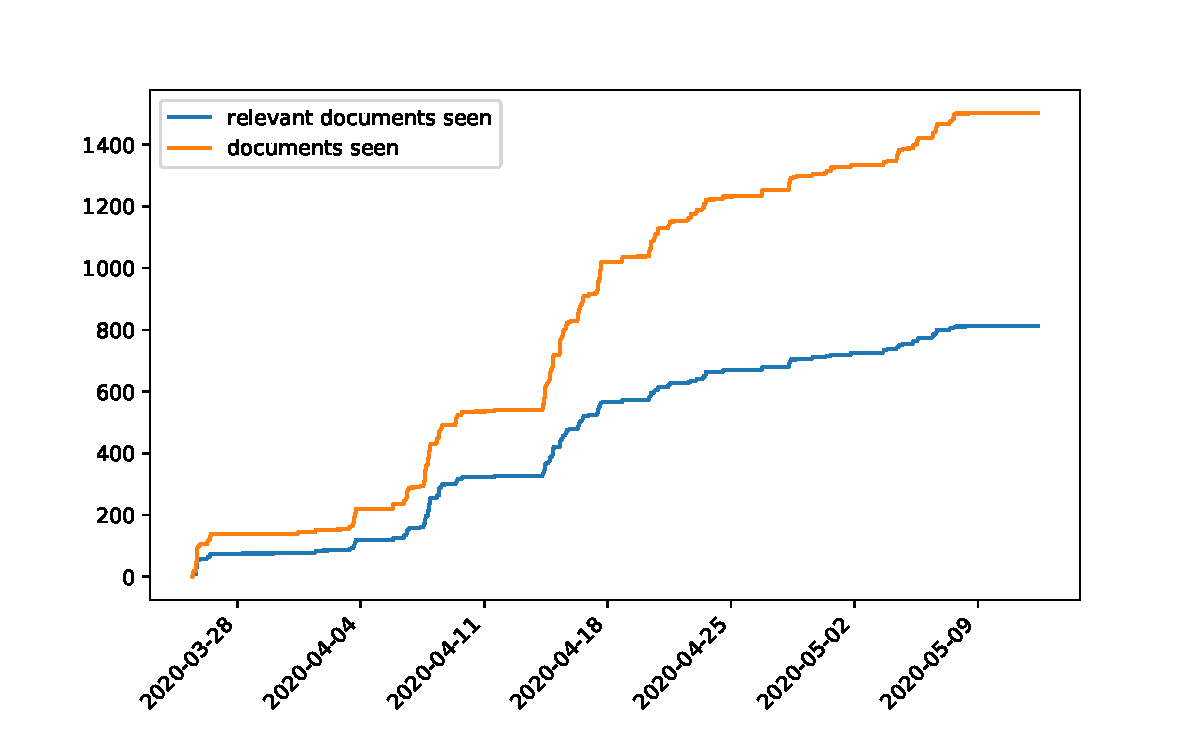
\includegraphics[width=\linewidth]{../plots/progress/docs_time.pdf}
\end{figure}

\only<2->{We're nearly at our target of 1500}

\end{frame}

\begin{frame}{We have already assembled a wealth of useful information}

\begin{figure}
	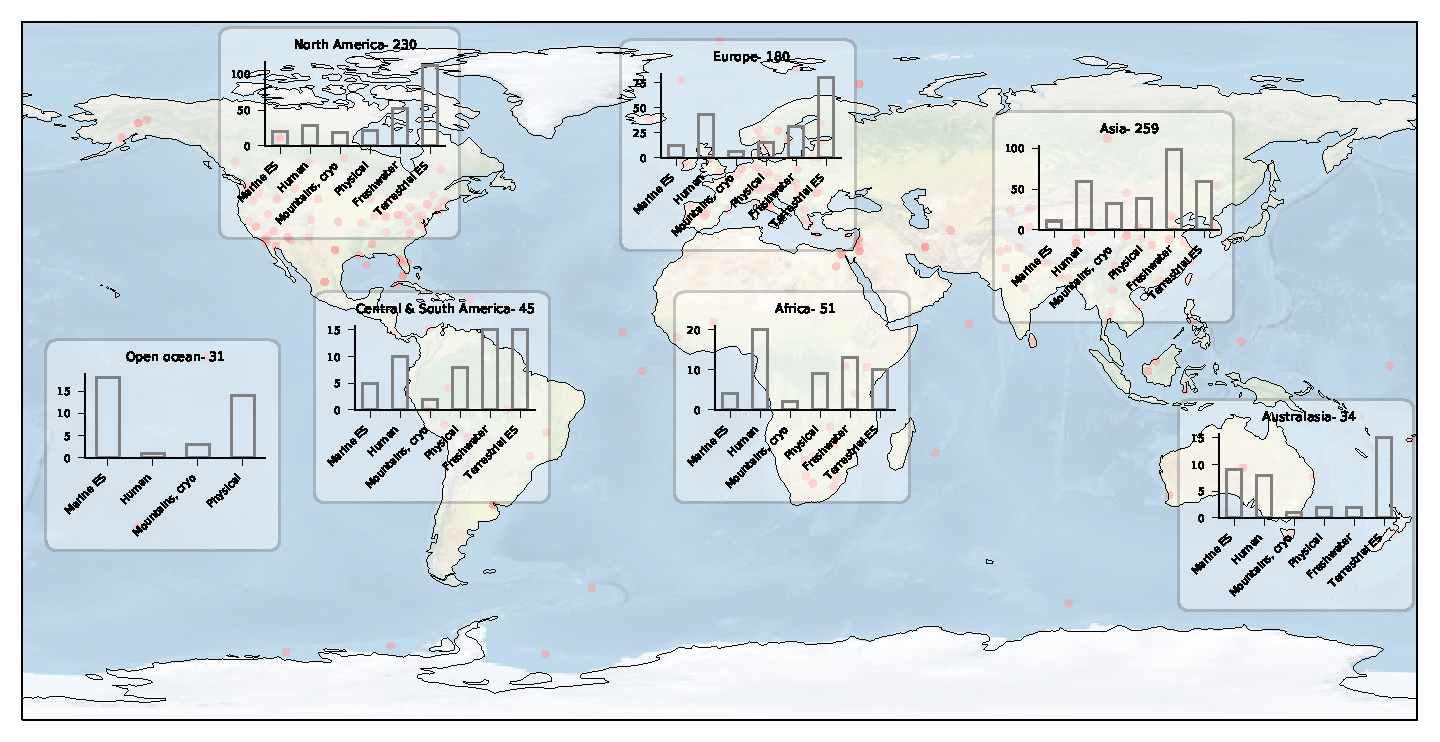
\includegraphics[width=\linewidth]{../plots/map_coded.pdf}
\end{figure}

\end{frame}

\begin{frame}{We can clearly identify what impact category a document is related to}

\begin{figure}
	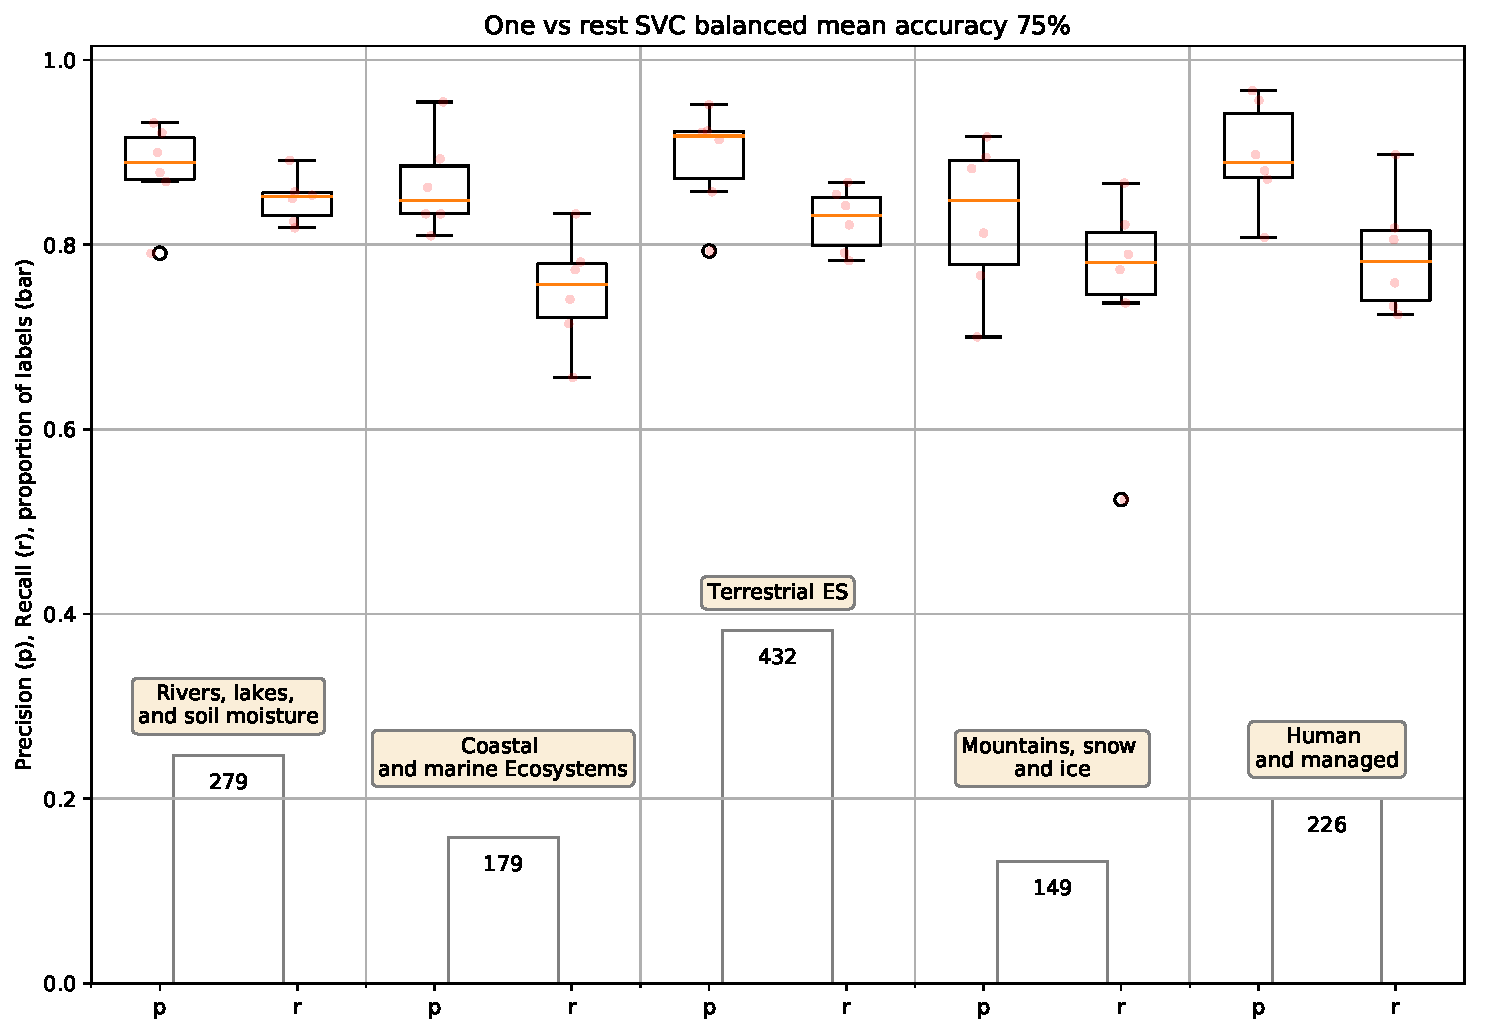
\includegraphics[width=0.9\linewidth]{../plots/progress/cats_prediction.pdf}
	\caption{Precision (how many documents predicted to be in a category actually had that label) and Recall (how many documents with a label were predicted to be in that category) for each broad impact category}
\end{figure}

\end{frame}

\begin{frame}{This is better than before because we have more labels, and we have investigated false negatives and false positives to find inconsistent labels}

\begin{figure}
	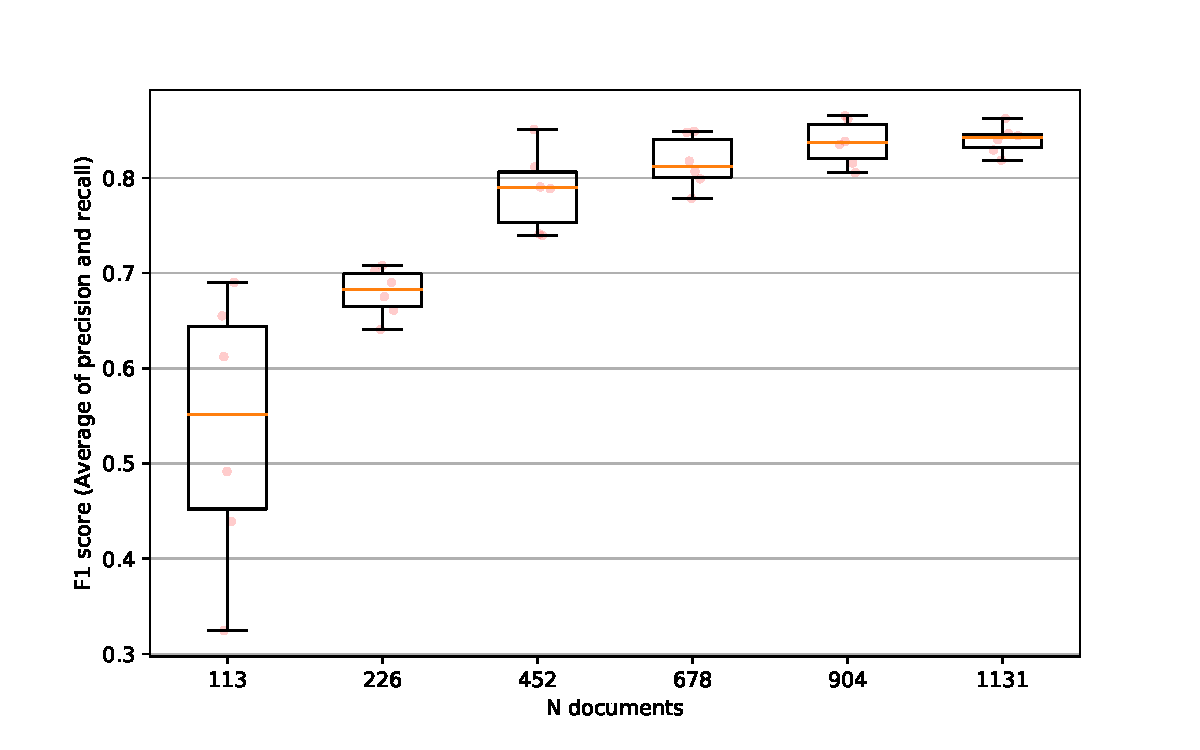
\includegraphics[width=0.8\linewidth]{../plots/progress/cats_prediction_n.pdf}
	\caption{Precision (how many documents predicted to be in a category were included by humans) and Recall (how many documents marked with a category by humans were predicted to have that category) for each broad impact category. The proportion of documents in each category is indicated with a bar, labelled with the absolute number of documents.}
\end{figure}

\end{frame}

\begin{frame}{We still have unbalanced subcategories, but we partially addressed this with the last samples}

\begin{itemize}
	\item Physical systems \hyperlink{Phy}{\beamergotobutton{subcategories}}
	\item Rivers, lakes and soil moisture \hyperlink{Riv}{\beamergotobutton{subcategories}}
	\item Mountains, snow and ice \hyperlink{Moun}{\beamergotobutton{subcategories}}
	\item Coastal and marine ecosystems \hyperlink{Mar}{\beamergotobutton{subcategories}}
	\item Terrestrial and freshwater ecosystems \hyperlink{TES}{\beamergotobutton{subcategories}}
	\item Human and managed systems \hyperlink{Hum}{\beamergotobutton{subcategories}}
\end{itemize}


\end{frame}

\begin{frame}{Plan}
\begin{figure}
	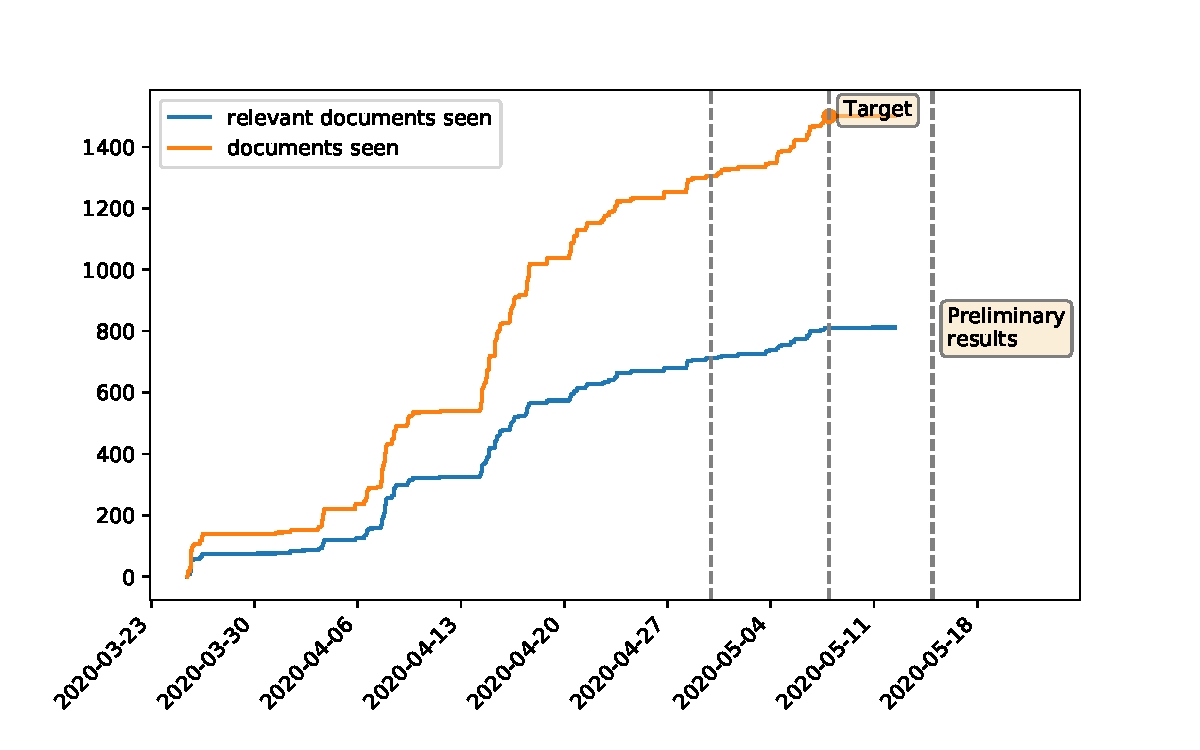
\includegraphics[width=\linewidth]{../plots/progress/plan.pdf}
\end{figure}
\end{frame}

\begin{frame}[label=Phy]{Physical systems}
\begin{figure}
	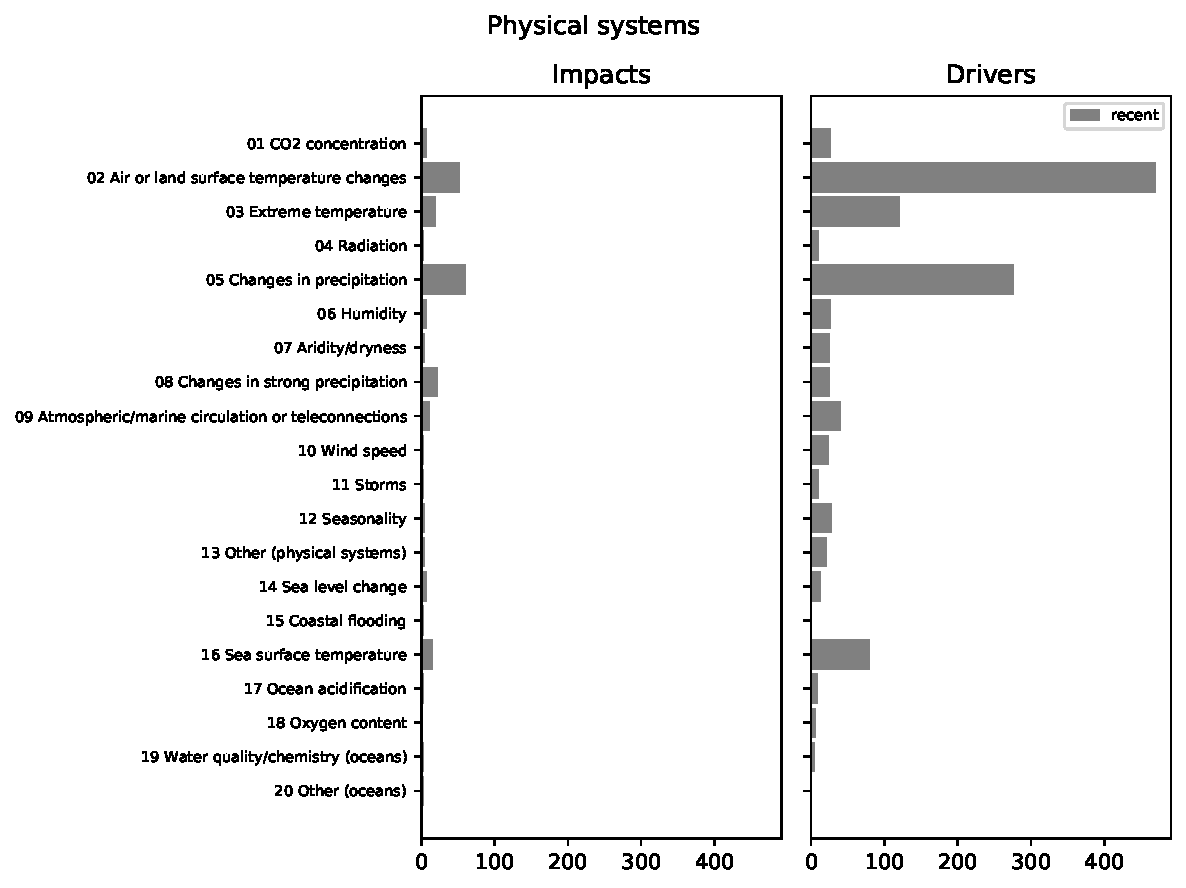
\includegraphics[width=\linewidth]{../plots/progress/cats_labels_Physical_systems.pdf}
\end{figure}
\end{frame}

\begin{frame}[label=Riv]{Rivers, lakes and soil moisture}
\begin{figure}
	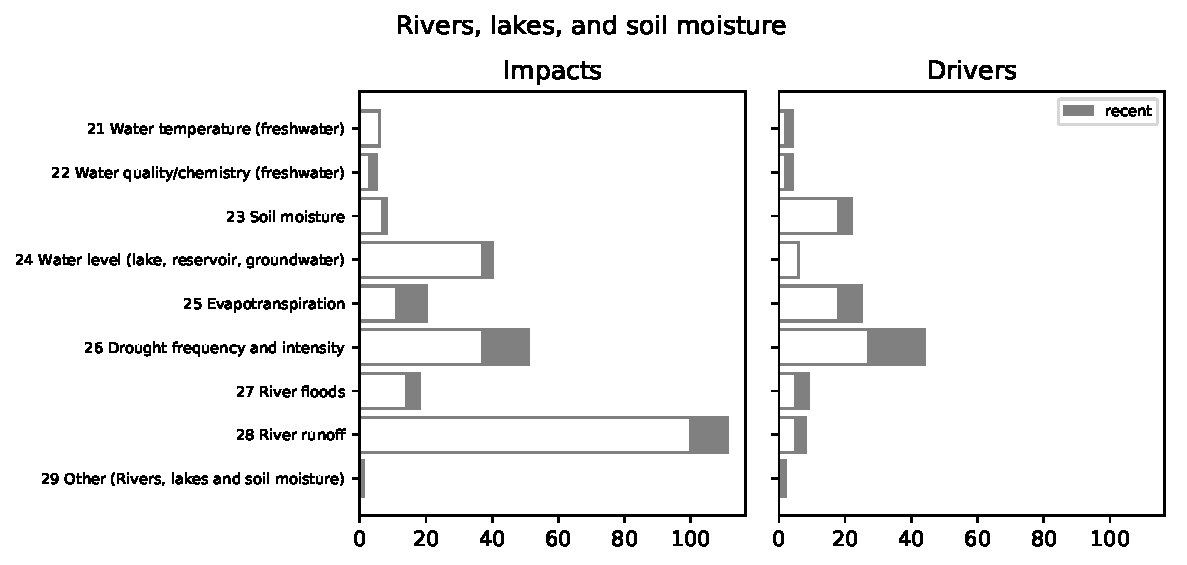
\includegraphics[width=\linewidth]{../plots/progress/cats_labels_Rivers,_lakes,_and_soil_moisture.pdf}
\end{figure}
\end{frame}

\begin{frame}[label=Moun]{Mountains, snow and ice}
\begin{figure}
	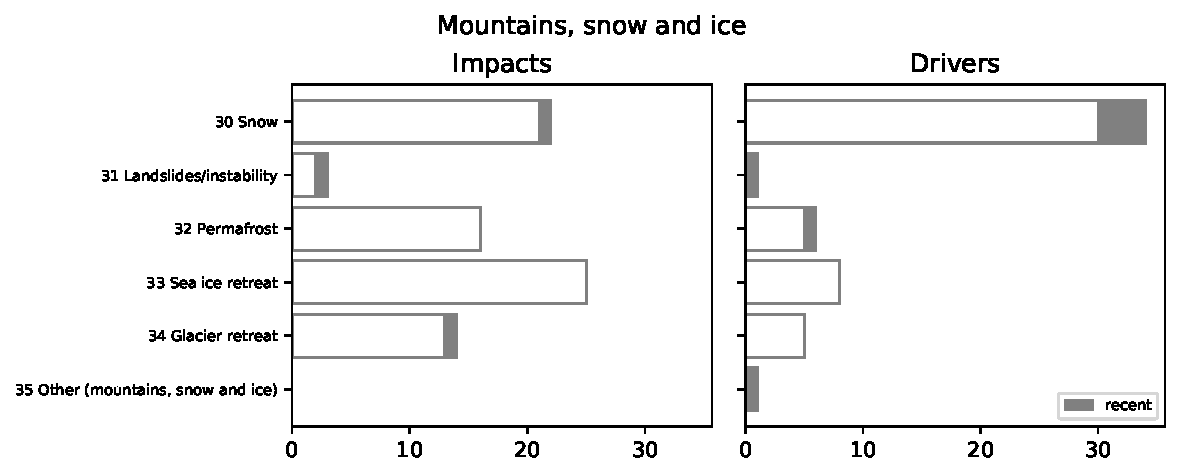
\includegraphics[width=\linewidth]{../plots/progress/cats_labels_Mountains,_snow_and_ice.pdf}
\end{figure}
\end{frame}


\begin{frame}[label=Mar]{Coastal and marine ecosystems}
\begin{figure}
	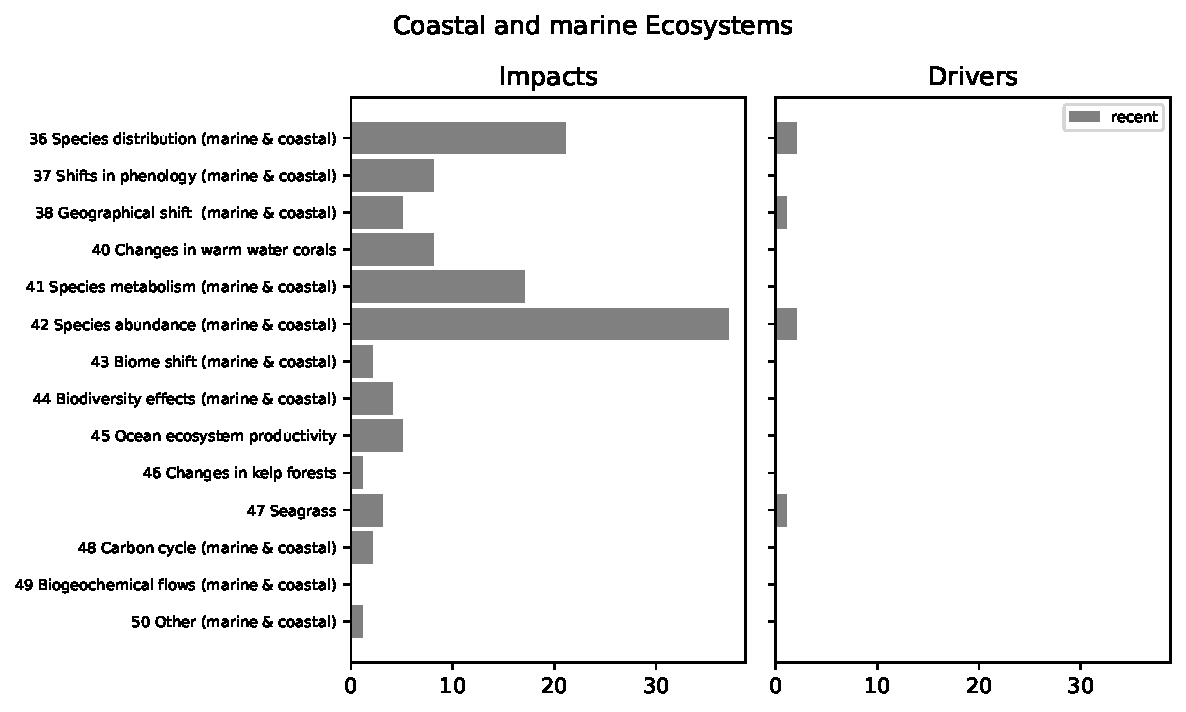
\includegraphics[width=\linewidth]{../plots/progress/cats_labels_Coastal_and_marine_Ecosystems.pdf}
\end{figure}
\end{frame}

\begin{frame}[label=TES]{Terrestrial and freshwater ecosystems}
\begin{figure}
	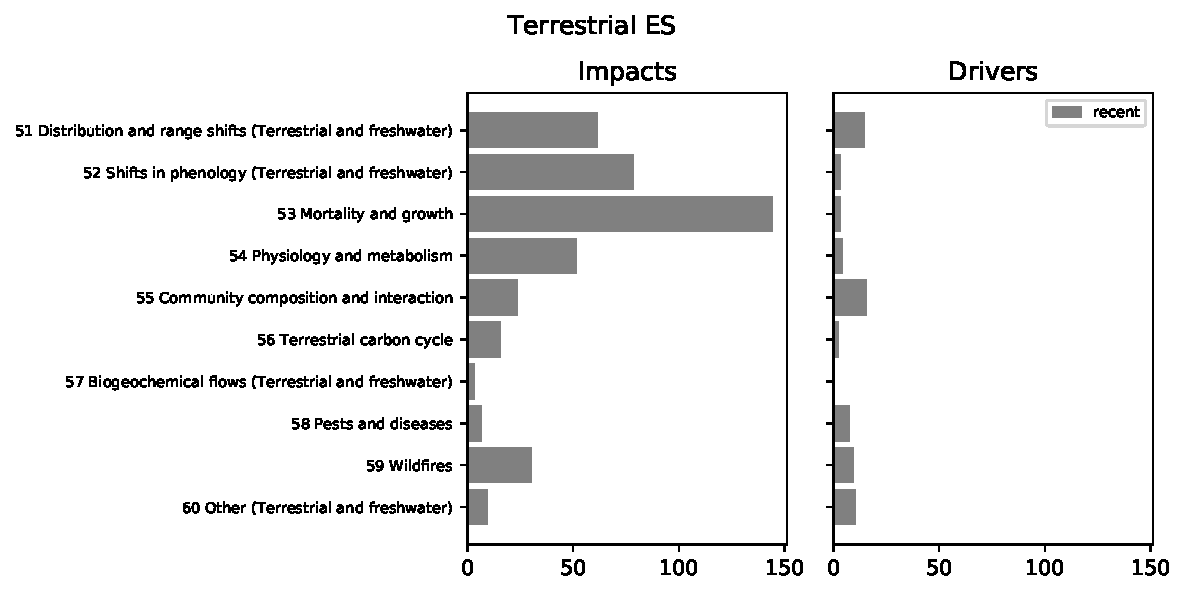
\includegraphics[width=\linewidth]{../plots/progress/cats_labels_Terrestrial_ES.pdf}
\end{figure}
\end{frame}

\begin{frame}[label=Hum]{Human and managed systems}
\begin{figure}
	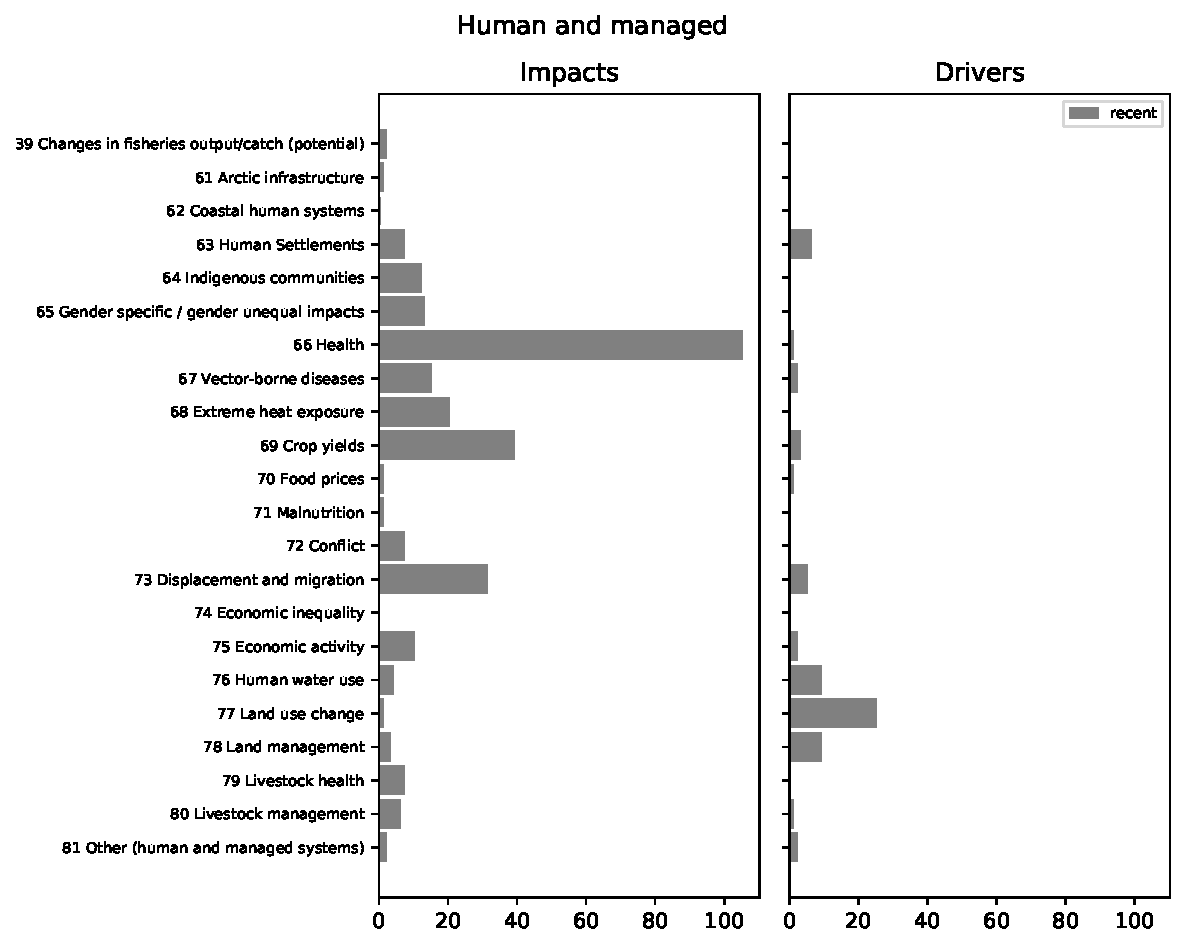
\includegraphics[width=\linewidth]{../plots/progress/cats_labels_Human_and_managed.pdf}
\end{figure}
\end{frame}

\end{document}